\section{Results: Multi-Antenna Devices}
\label{sec:results-multi}

% src: seed_repeats_all_models_summary.json per_config.*_h0/_h5 runs (seed-paired multi_mae differences, computed per seed; CI = 1.96 sd / sqrt(5))
For multi-antenna devices, history lowered error in every one of the seven model families, by $2.8$ to $4.1\,\text{m}$, or $15$ to $21\%$ of each model's own $h=0$ error~(Figure~\ref{fig:history-gain-ci}; per-model values in Table~\ref{tab:history-gain}). Each gain is a seed-paired difference over five independent user splits, and none of the seven confidence intervals comes close to zero. The gain is of similar size across instance-based, bagged, boosted, recurrent, convolutional and attention-based models, which is the behavior expected if history supplies information that the $h=0$ input lacks, rather than suiting one architecture's inductive bias. These gains are measured under the angle impairment of Section~\ref{sec:setup}, in which every report carries an independent $4^\circ$ error; Section~\ref{subsec:averaging} shows how much of the gain depends on that.

\begin{figure}[h]
  \centering
  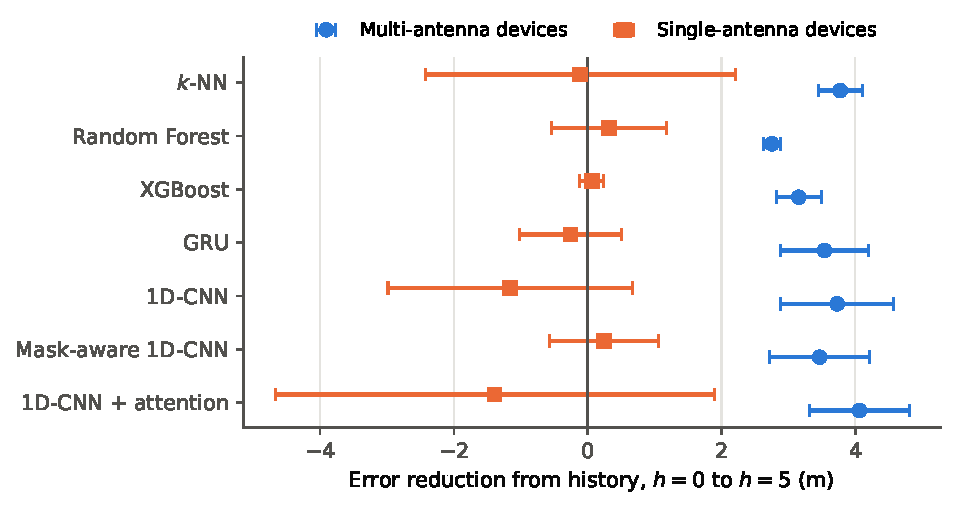
\includegraphics[width=0.8\textwidth]{fig_history_gain_ci}
  \caption{Reduction in mean error from adding history~($h=0$ to $h=5$), per model and device group, macro-cell study. Each marker is the mean seed-paired difference over five user splits; bars are $95\%$ confidence intervals. Positive values mean history lowered the error.}
  \label{fig:history-gain-ci}
\end{figure}
% src: figure_scripts/make_figures.py history_gain_ci(); seed_repeats_all_models_summary.json

% src: history_sweep_all_models_summary.json curves (seed 42, multi_mae by depth)
The gain builds over the first few steps of history and then levels off~(Figure~\ref{fig:history-by-group}, left). With the exception of $k$-NN, whose error rises again between $h=5$ and $h=10$, and Random Forest, which is flat over that interval, every family is still improving at $h=10$, or $40\,\text{m}$ of travel. For XGBoost the overall error varies by only about $0.05\,\text{m}$ between $h=10$ and $h=30$. In follow-up runs over $10$ to $20$ user splits, XGBoost's gain from the full window is $1.2$, $2.5$, $3.2$, $3.5$ and $3.7\,\text{m}$ at $1$, $3$, $5$, $10$ and $20$ steps, so most of it is in place by $10$ steps. No single depth is optimal across families; what distinguishes them is whether an over-long window costs anything. A tree ensemble can decline to split on an uninformative lag, whereas $k$-NN measures distance over the whole concatenated window, so each stale lag adds noise to its metric; this account is offered as an interpretation of the depth curves rather than as a separately tested result.
% src: deep_history_sweep_trees_summary.json (XGBoost h=10..30 spread 0.053 m); FINAL_REPORT.md §5.4

\begin{figure}[h]
  \centering
  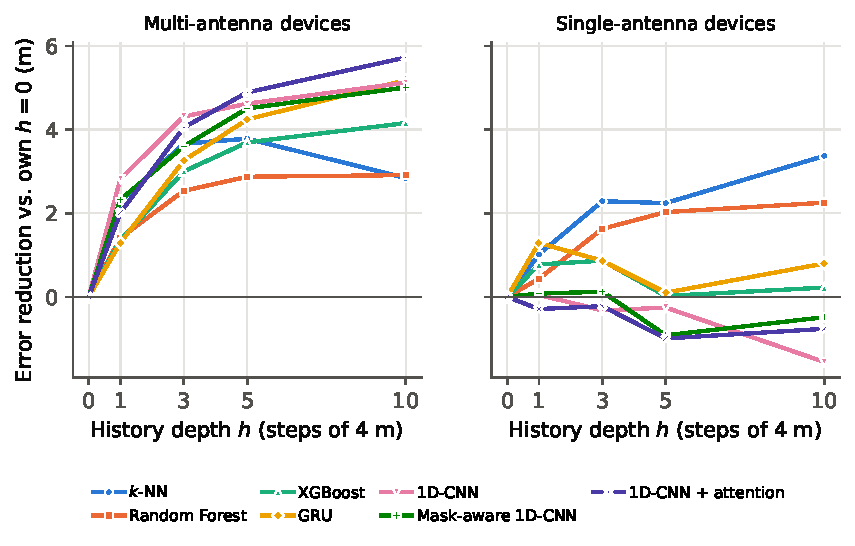
\includegraphics[width=0.9\textwidth]{fig_history_by_group}
  \caption{Error reduction against each model's own $h=0$ input as history depth grows, macro-cell study. Each step of history is $4\,\text{m}$ of travel. Single seed; the single-antenna curves move within that group's seed-to-seed spread, and the five-seed paired values at $h=5$ are those of Figure~\ref{fig:history-gain-ci}.}
  \label{fig:history-by-group}
\end{figure}
% src: figure_scripts/make_figures.py history_by_group(); history_sweep_all_models_summary.json

% src: history_by_speed_class_summary.json by_model.cnn (seed 42; best h 10/10/5/5 for static/pedestrian/jogger/vehicle; windows 134.7/31.0/7.1/1.6 s); FINAL_REPORT.md §5.8 (7-18 test users per class)
Because each step covers one grid cell, history depth measures distance travelled rather than elapsed time, and the speed classes of the population separate the two~(Figure~\ref{fig:speed-classes}). Measured against path length, the four classes improve over a similar span: every class has gained most of its benefit within $12$ to $20\,\text{m}$. Measured against time, the same curves are spread across two orders of magnitude, and the 1D-CNN's best window lasts $1.6\,\text{s}$ for vehicles but $135\,\text{s}$ for near-static users. The useful window is therefore set by how far a device has moved through the spatially consistent channel, not by how long it took to do so. Vehicles gain least, about $4\%$ against $17$ to $28\%$ for the other classes. Each class contains only $7$ to $18$ test users, so these are single-seed indications, and because step length is fixed in these simulations, the number of samples and the distance covered cannot be separated.

\begin{figure}[h]
  \centering
  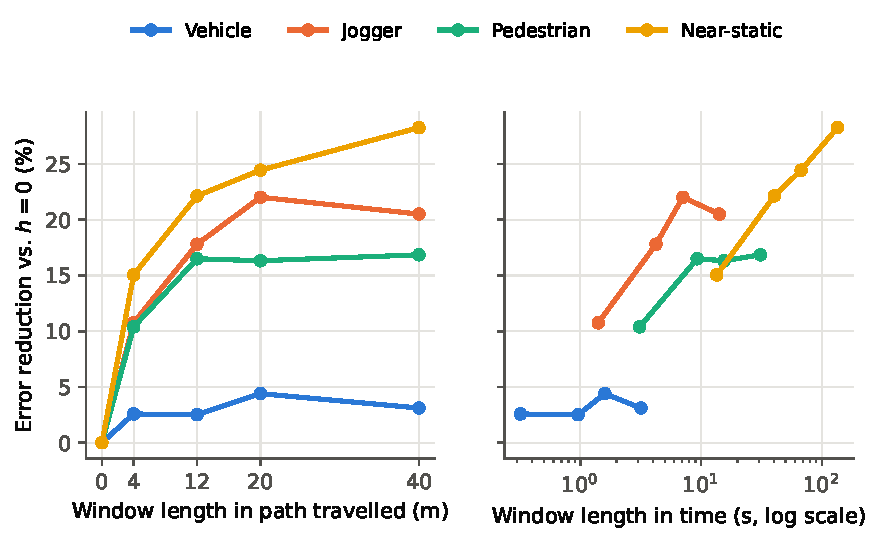
\includegraphics[width=0.85\textwidth]{fig_speed_classes}
  \caption{Error reduction against $h=0$ for each speed class, 1D-CNN, macro-cell study, plotted against the window's length in path travelled~(left) and in time~(right, logarithmic). Points correspond to $h=0$, $1$, $3$, $5$ and $10$. Single seed, $7$ to $18$ test users per class.}
  \label{fig:speed-classes}
\end{figure}
% src: figure_scripts/make_figures.py speed_classes()

% src: xgb_per_h_retune_summary.json and rf_per_h_retune_summary.json: XGBoost tuning buys <= 0.44 m; RF tuning moves -0.046 to +0.066 m
Two checks rule out the most direct alternative explanations. A larger input could help simply because fixed hyperparameters happen to suit it better, so XGBoost and Random Forest were re-tuned separately at every depth, on training users only. Re-tuning changed XGBoost's error by at most $0.44\,\text{m}$ and Random Forest's by less than $0.07\,\text{m}$, and the history gain was essentially unchanged~(Table~\ref{tab:supp-retune}). The derived input channels also matter less than history: replacing them with the five raw channels raised the 1D-CNN's error at $h=5$ by $0.43\,\text{m}$ in a single run, a difference that is suggestive but small beside the gain from history.
% src (feature ablation): FINAL_REPORT.md §5.2 (19.686 raw vs 19.260 derived, 1D-CNN, h=5)

% src: seed_repeats_all_models_summary.json ranking (h=5 overall, ranks 1-6 18.810-19.275, all adjacent pairs overlapping); master_benchmark_rerun_summary.json (cost)
With history in place, the choice of model matters far less than the input. At $h=5$ the six trained models other than $k$-NN fall within $0.47\,\text{m}$ of each other in overall error, with overlapping confidence intervals for every adjacent pair. XGBoost reaches that level in $4\,\text{s}$ of training and predicts $1000$ positions in a few milliseconds ($1.7\,\text{ms}$ in one timing and $8.3\,\text{ms}$ in another), and the neural models' errors are, if anything, flattered by their test-based stopping rule. A small boosted-tree ensemble therefore collects the full benefit of history at a fraction of the cost.

% src: rts_retune_all_models_summary.json (best RTS gains: RF 2.49, XGB 4.35, 1D-CNN 3.65, GRU 3.72, attention 4.74%); trajectory_diagnostics_summary.json via FINAL_REPORT.md §7.7 (forward Kalman 19.13 -> 19.77 m, 1D-CNN)
Temporal information can also be used after the estimator rather than inside it. A Rauch--Tung--Striebel~(RTS) smoother applied to the trained models' predicted tracks lowered their error by a further $2.5$ to $4.7\%$, but with two qualifications: the smoother's noise parameters were tuned on the test users, and its gain comes entirely from the backward pass, which uses future samples. Running only the forward filter raised the 1D-CNN's error by $3.4\%$. Smoothing is thus a complement to history for offline track reconstruction, whereas history uses past samples only and is available in real time.

% Hand-off to the single-antenna section
All of these gains belong to devices that report an angle. Single-antenna devices are the ones that face the distance-ring ambiguity in its pure form, and they are where history would be expected to matter most.
